
\chapter{WAVESHAPING}
\title{Sintesi e Sistemi Non Lineari}

\section{Sintesi Additiva}
Molto onerosa a livello computazionale.

Con una sintesi FM si possono ottenere spettri più ricchi e complessi.

\section*{Waveshaping}
Si ottiene uno spettro complesso tramite dispersione.

\section{Sistemi Non Lineari}

Due categorie:
\begin{itemize}
    \item \textbf{Con memoria}:
    \begin{itemize}
        \item descritti con una rappresentazione in spazio di stato:
        \[
        \begin{cases}
        z'(x) = f(t, z(t), x(t)) \\
        y(t) = g(t, z(t), x(t))
        \end{cases}
        \]
    \end{itemize}
    
    \item \textbf{Senza memoria (statici)}:
    \begin{itemize}
        \item $y = f(x)$ dove l’input $x$ può essere un segnale del tempo: $y(t) = f(x(t))$
        \item la conoscenza della funzione $f(x)$ è rappresentativa del sistema, ad esempio:
        \begin{itemize}
            \item $f(x) = \tanh(x)$
            \item $f(x) = \sum_{p=0}^{N} a_p x^p$
            \item ecc.
        \end{itemize}
    \end{itemize}
\end{itemize}

\begin{figure}[H]
    \centering
    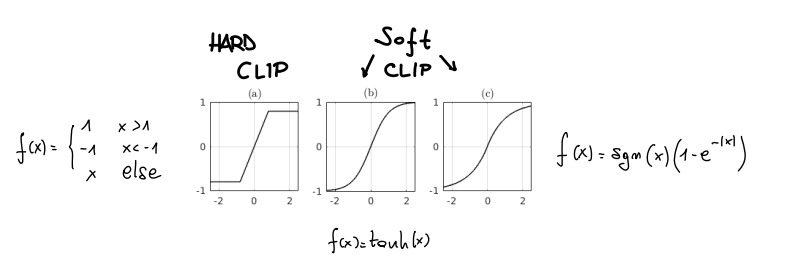
\includegraphics[width=0.7\textwidth]{capitoli/capitolo11/immagini/image1.png}
\end{figure}

\section*{Effetto di Termini Moltiplicativi}

Una moltiplicazione può avere effetti differenti in base alla regione in cui si trova:
\begin{itemize}
    \item Regione quasi lineare $\rightarrow$ semplice moltiplicazione
    \item Regione non lineare $\rightarrow$ effetto molto grande sull’uscita del sistema
\end{itemize}

\section{Effetto di Termini Additivi}

Aggiungendo un termine costante all’ingresso prima della non linearità si ottiene un effetto simile allo spostamento della funzione non lineare.

\section*{Armoniche Pari e Dispari}

\begin{itemize}
    \item Funzioni dispari $\rightarrow$ generano solo armoniche dispari
    \item Funzioni pari $\rightarrow$ generano solo armoniche pari che annullano la fondamentale
    \item Le altre funzioni possono generare qualsiasi tipo di armonica
\end{itemize}

\section{Distorsione}

Funzione non lineare approssimata tramite espansione polinomiale:
\[
y(t) = a_0 + a_1 x + a_2 x^2 + \cdots + a_N x^N
\]

Per valutare l’effetto di distorsione di un segnaloo con un sato polinomio:
\begin{figure}[H]
    \centering
    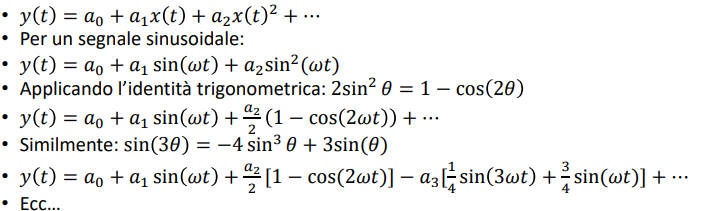
\includegraphics[width=0.7\textwidth]{capitoli/capitolo11/immagini/image2.png}
\end{figure}

\section*{Intermodulazione}

Si consideri un sistema non lineare in cui $f(x_1 + x_2) \neq f(x_1) + f(x_2)$.

\subsection*{1. Espansione non lineare}

\[
y(t) = a_0 + a_1 x(t) + a_2 x(t)^2 + \dots
\]

\subsection*{2. Due segnali sinusoidali in ingresso}

\[
x(t) = \sin(\omega_1 t) + \sin(\omega_2 t)
\]

\[
y(t) = a_0 + a_1[\sin(\omega_1 t) + \sin(\omega_2 t)] + a_2[\sin(\omega_1 t) + \sin(\omega_2 t)]^2 + \dots
\]

\subsection*{3. Sviluppo del termine quadratico}

\[
[\sin(\omega_1 t) + \sin(\omega_2 t)]^2 = \sin^2(\omega_1 t) + \sin^2(\omega_2 t) + 2\sin(\omega_1 t)\sin(\omega_2 t)
\]

Risultano:
\begin{itemize}
    \item \textbf{Componenti armoniche superiori}: $\sin^2(\omega_1 t)$ e $\sin^2(\omega_2 t)$ generano frequenze raddoppiate.
    \item \textbf{Prodotti di intermodulazione}: $\sin(\omega_1 t) \sin(\omega_2 t)$ produce nuove frequenze somma e differenza, come $\omega_1 + \omega_2$ e $\omega_1 - \omega_2$.
\end{itemize}

\subsection*{Conclusioni}

\begin{itemize}
    \item Due segnali sinusoidali in un sistema non lineare generano nuove frequenze.
    \item Frequenze: armoniche superiori e combinazioni $(\omega_1 + \omega_2, \omega_1 - \omega_2)$.
    \item Fenomeno rilevante in elettronica, telecomunicazioni e audio (distorsione indesiderata).
\end{itemize}

\subsection*{Misure}
\begin{itemize}
    \item \textbf{Total Harmonic Distortion (THD)}:
    \[
    THD_F = \frac {\sqrt{V_2^2 + V_3^2 + V_4^2 + \cdots}}{V_1}
    \]
    
    \item \textbf{Signal to Noise Ratio (SNR)}:
    \[
    SNR = \frac{P_{signal}}{P_{noise}}
    \]
    misura la potenza di tutte le parziali inarmoniche.
\end{itemize}

\section{Waveshaping}

\begin{itemize}
    \item utilizza una non linearità applicata a una forma d’onda semplice
    \item semplice e poco costosa
    \item crea spettri complessi
    \item la sintesi FM è un caso particolare di WS
    \item ogni forma d’onda periodica è vista come un seno mandato in una non linearità
    \item spettri che variano nel tempo si possono ottenere moltiplicando l’ingresso per un EG (Envelope Generator)
\end{itemize}

\section*{Look-Up Table (LUT)}

\begin{itemize}
    \item utilizzate in applicazioni di calcolo del suono e della musica
    \item tabella di valori precalcolati (array in memoria)
    \item per ottenere valori intermedi si interpola
    \item basso costo computazionale
    \item la memoria può ridurre le prestazioni (letture frequenti)
    \item le approssimazioni producono errori come distorsione armonica
\end{itemize}

\section*{Aliasing}

\begin{itemize}
    \item funzioni non lineari o clipping generano espansione di banda
    \item nei segnali a tempo discreto si rischia aliasing
    \item si può usare l’oversampling per evitarlo
\end{itemize}

\section*{Wavefolding}

\begin{itemize}
    \item tipo particolare di waveshaping
    \item la funzione non lineare “ribalta” la forma d’onda invece che clipparla o distorcerla
\end{itemize}

\begin{figure}[H]
    \centering
    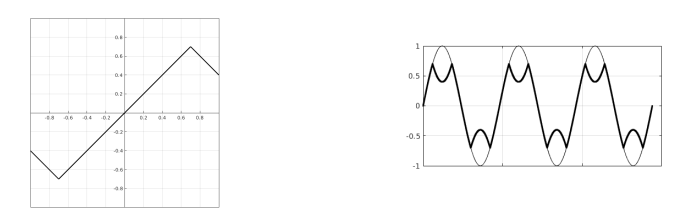
\includegraphics[width=0.7\textwidth]{capitoli/capitolo11/immagini/image3.png}
\end{figure}
